\chapter{Gegevensstructuren voor strings}
\section{Inleiding}
\begin{itemize}
    \item Efficiënte gegevensstructuren kunnen een zoeksleutel lokaliseren door elementen één voor één te testen.
    \item Dit heet \textbf{radix search}.
    \item Meerdere soorten boomstructuren die radix search toepassen.
    \alert Veronderstel dat geen enkele sleutel een prefix is van een ander.

    De sleutels \texttt{test} en \texttt{testen} zullen dus nooit samen voorkomen in de boom aangezien \texttt{test} een prefix is van \texttt{testen}.
\end{itemize}

\section{Digitale zoekbomen}
\begin{itemize}
    \item Sleutels worden opgeslagen in de knopen.
    \item Zoeken en toevoegen verloopt analoog.
    \item Slechts één verschil:
    \begin{itemize}
        \item De juiste deelboom wordt niet bepaald door de zoeksleutel te vergelijken met de sleutel in de knoop.
        \item Wel door enkel het volgende element (van links naar rechts) te vergelijken.
        \item Bij de wortel wordt het eerste sleutelelement gebruikt, een niveau dieper het tweede sleutelelement, enz.
    \end{itemize}
    \item Hier zijn de sleutelelementen beperkt tot bits $\rightarrow$ \textbf{binaire digitale zoekbomen}.
    \item Bij een knoop op diepte $i$ wordt bit $(i + 1)$ van de zoeksleutel gebruikt om af te dalen in de juiste deelboom.
    \alert De zoeksleutels zijn niet noodzakelijk in volgorde van toevoegen.
    \begin{itemize}
        \item Sleutels in de linkerdeelboom van een knoop op diepte $i$ zijn kleiner dan deze in de rechterdeelboom, maar \todo{wat?}
    \end{itemize}
    \item De hoogte van een digitale zoekboom wordt bepaald door het aantal bits van de langste sleutel.
    \item Performantie is vergelijkbaar met rood-zwarte bomen:
    \begin{itemize}
        \item Voor een groot aantal sleutels met relatief kleine bitlengte is het zeker beter dan een binaire zoekboom en vergelijkbaar met die van een rood-zwarte boom.
        \item Het aantal vergelijkingen is trouwens nooit meer dan het aantal bits van de zoeksleutel.
        \good Implementatie van een digitale zoekboom is eenvoudiger dan die van een rood-zwarte boom.
        \alert De beperkende voorwaarde is echter dat er efficiënte toegang nodig is tot de bits van de sleutels.
    \end{itemize}
\end{itemize}

\section{Tries}
\begin{itemize}
    \item Een digitale zoekstructuur die wel de volgorde van de opgeslagen sleutels behoudt.
\end{itemize}

\subsection{Binaire tries}

\begin{figure}[ht]
    \centering
    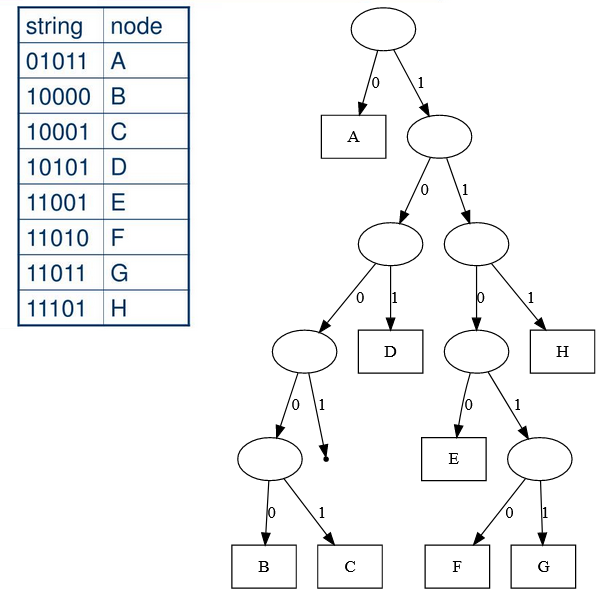
\includegraphics[width=\textwidth]{binary_trie}
    \caption{Een voorbeeld van een binaire trie met opgeslagen sleutels $A$, $B$, $C$, $D$, $E$, $F$, $G$ en $H$. Elk van deze sleutels heeft een (willekeurige) bitrepresentatie die de individuele elementen van de sleutels voorstelt. De zoekweg van de sleutel $E$ wordt aangegeven door rode verbindingen.}
    \label{fig:binary_trie}
\end{figure}

\begin{itemize}
    \item Zoekweg wordt bepaald door de opeenvolgende bits van de zoeksleutel.
    \item Sleutels worden enkel opgeslaan in de bladeren.
    \begin{itemize}
        \item  De boom \textit{inorder} overlopen geeft de sleutels gerangschikt terug.
        \item  De zoeksleutel moet niet meer vergeleken worden met elke knoop op de zoekweg. 
    \end{itemize}
    \item Twee mogelijkheden bij \textbf{zoeken} en \textbf{toevoegen}:
    \begin{enumerate}
        \item Indien een lege deelboom bereikt wordt, bevat de boom de zoeksleutel niet. De zoeksleutel kan dan in een nieuw blad op die plaats toegevoegd worden.
        \item Anders komen we in een blad. De sleutel in dit blad \textbf{kan} eventueel gelijk zijn aangezien ze zeker dezelfde beginbits hebben.  

        \begin{itemize}
            \item Als we bijvoorbeeld \texttt{testen} zoeken maar de boom bevat enkel de sleutel \texttt{test}, zullen we in het blad met de sleutel \texttt{test} uitkomen aangezien de eerste 4 elementen hetzelfde zijn. De sleutels zijn echter niet gelijk.
            \item Indien de sleutels niet hetzelfde zijn, zijn er terug twee mogelijkheden:
            \begin{enumerate}
                \item \textbf{Het volgende bit verschilt.} Het blad wordt vervangen door een knoop met twee kinderen die de twee sleutels bevat.
                \item \textbf{Een reeks van opeenvolgende bits is gelijk.} Het blad wordt vervangen door een reeks van inwendige knopen, zoveel als er gemeenschappelijke bits zijn. Bij het eerste verschillende krijgen we terug het eerste geval.
            \end{enumerate}
        \end{itemize}
    \end{enumerate}
    \alert Wanneer opgeslagen sleutels veel gelijke bits hebben, zijn er veel knopen met één kind.
    \begin{itemize}
        \item Het aantal knopen is dan ook hoger dan het aantal sleutels.
        \item Een trie met $n$ gelijkmatige verdeelde sleutels heeft gemiddeld $n/\ln 2 \approx 1.44n$ inwendige knopen.
    \end{itemize}
    \item De structuur is onafhankelijk van de toevoegvolgorde van de sleutels.
    \item De sleutels in de zoekweg worden enkel getest op de bit die op dat niveau van toepassing is.
\end{itemize}


\subsection{Meerwegstries}
\begin{itemize}
    \item Heeft als doel de hoogte van een trie met lange sleutels te beperken.
    \item Meerdere sleutelbits in één enkele knoop vergelijken.
    \item Een sleutelelement kan $m$ verschillende waarden aannemen, zodat elke knoop (potentiaal) $m$ kinderen heeft $\rightarrow$ $m$-wegsboom.
\end{itemize}